%++++++++++++++++++++++++++++++++++++++++
% Don't modify this section unless you know what you're doing!
%\documentclass[letterpaper,12pt]{article}
\documentclass[14pt]{extarticle}
%\documentclass[journal, a4paper]{IEEEtran}
\usepackage{tabularx} % extra features for tabular environment
\usepackage{amsmath}  % improve math presentation
\usepackage{graphicx} % takes care of graphic including machinery
\usepackage[margin=1in,letterpaper]{geometry} % decreases margins
\usepackage{cite} % takes care of citations
\usepackage[final]{hyperref} % adds hyper links inside the generated pdf file
%\usepackage{mathtext}
\hypersetup{
	colorlinks=true,       % false: boxed links; true: colored links
	linkcolor=blue,        % color of internal links
	citecolor=blue,        % color of links to bibliography
	filecolor=magenta,     % color of file links
	urlcolor=blue         
}
\usepackage{textcomp}
\usepackage{ gensymb }
\usepackage{latexsym}
\usepackage{geometry} % пакет для установки полей
\geometry{top=1.5cm} % отступ сверху
\geometry{bottom=2cm} % отступ снизу
\geometry{left=3cm} % отступ справа
\geometry{right=1cm} % отступ слева
\usepackage{amsfonts}
\newcommand*{\No}{\textnumero}
\renewcommand{\Re}{\mathrm{Re}}
\renewcommand{\Im}{\mathrm{Im}}

\newcommand{\const}{\mathrm{const}}
\newcommand{\arccosh}{\mathrm{arccosh}}
%++++++++++++++++++++++++++++++++++++++++

\usepackage[T2A]{fontenc}
\usepackage[utf8]{inputenc}
\usepackage[english, russian]{babel}

\begin{document}

\begin{center}
	\hfill \break
	\large{МИНОБРНАУКИ РОССИИ}\\
	\footnotesize{ФЕДЕРАЛЬНОЕ ГОСУДАРСТВЕННОЕ БЮДЖЕТНОЕ ОБРАЗОВАТЕЛЬНОЕ УЧРЕЖДЕНИЕ}\\
	\footnotesize{ВЫСШЕГО ПРОФЕССИОНАЛЬНОГО ОБРАЗОВАНИЯ}\\
	\small{\textbf{«ВОРОНЕЖСКИЙ ГОСУДАРСТВЕННЫЙ УНИВЕРСИТЕТ»}}\\
	\hfill \break
	\normalsize{Факультут Компьютерных наук}\\
	\hfill \break
	\normalsize{Кафедра Цифровых технологий}\\
	\hfill\break
	\hfill \break
	\hfill \break
	\hfill \break
	\large{Метод превала.\\ Аппроксимация функции Бесселя}\\
	\hfill \break
	\hfill \break
	\hfill \break
	\normalsize{Курсовая работа\\
		\hfill \break
		02.03.01 Математика и компьютерные науки\\
		\hfill \break
		Распределенные системы и искусственный интеллект}\\
	\hfill \break
	\hfill \break
\end{center}

\hfill \break
\hfill \break

\normalsize{
	\begin{tabular}{cccc}
		Зав.кафедрой & \underline{\hspace{3cm}} &  д.физ.-мат.н.,  проф. & С.Д. Кургалин \\\\
		Студент & \underline{\hspace{3cm}} & &А.А. Махно \\\\
		Руководитель & \underline{\hspace{3cm}}& канд.физ.-мат.н, доц.&  А.В. Флегель \\\\
	\end{tabular}
}\\
\hfill \break
\hfill \break
\begin{center} Воронеж 2016 \end{center}
\thispagestyle{empty} % выключаем отображение номера для этой страницы

\newpage	
\tableofcontents
\thispagestyle{empty} % выключаем отображение номера для этой страницы
\newpage	
\section{Введение}
В наше время, при различного вида научных исследований, возникает необходимость использования численных методов. Лишь малое количество интересующих нас функций имеют аналитическую форму. Несмотря на наличие большого количества хороших численных вычислений, так или иначе, возникает проблема скорости. Предположим, мы должны выполнить какое-то исследование, результаты которого остаются актуальными в течении 10 часов, но для этого нужно решить систему дифференциальных уравнений, на решение которой, даже численного, уходит 2 дня. 

Да, есть способы ускорить этот процесс, повысив производительность вычислительной машины, усовершенствованием параллельного алгоритма, и т. п. Но в большинстве случаев такой возможности нет. Также если речь заходит о том, чтобы варьировать параметры системы, и сравнивать изменения, то некоторые методы могут работать не очень хорошо. Проблематично исследовать зависимость от параметров, если на численное решение от одного только набора уходит несколько суток. 

Поэтому имеет смысл перейти от "тяжелых" численных методов к приближенным оценкам.

Целью данной курсовой работы является посмотреть на одну из таких оценок, а именно на Метод перевала, который входит в семейство перевальных оценок. Основной идеей этих оценок является изменение контура интегрирования таким образом, чтобы он в первую очередь, проходил через так называемые седловые точки. Мы посмотрим на границы его применимости, приведем в виде примера аппроксимацию одного из интегралов Бесселя, и исследуем полученную оценку на различных участках. Конечно, данный метод применим к гораздо большему чилу интегралов, но интеграл Бесселя я выбрал потому, что функция Бесселя (для первого рода) хорошо известна и может быть легко вычислена в любом математическом пакете. Именно эта "известность" поможет нам оценить погрешности и причины их возникновения на разных участках интегрирования. 

Сначала я расскажу о том, что такое вообще функции Бесселя и где они применяются, а также, самое главное для нас - их интегральные формы . Затем мы рассмотрим идею метода перевала, представляющего собой Метод Лапласа, но расширенный до комплексно-значимой плоскости, докажем, что это расширение возможно. Получив готовую формулу для вычисления интегралов вида (\ref{eq:eq6}), попробуем вычислить интеграл Бесселя, и в завершение построим полученную оценку и сравним его с исходным интегралом. 


\section{Функции Бесселя}
Имеется дифференциальное уравнение вида:
\begin{equation}\label{eq:eq4}
x^2\frac{d^2 y}{dx^2}+x\frac{dy}{dx}+(x^2-\alpha^2)y = 0,
\end{equation}
где $\alpha$ - произвольное вещественное число (в общем случае комплексное), называемое порядком. Чаще всего речь идет о целых порядках.

Решением таких уравнений являются функции Бесселя.
Они используются при решении множества задач, где используется переход в цилиндрические и сферические координаты, например:
\begin{itemize}
	\item электромагнитные волны в цилиндрическом волноводе;
	\item теплопроводность в цилиндрических объектах;
	\item формы колебания тонкой круглой мембраны
	\item распределение интенсивности света, дифрагированного на круглом отверстии.
	\item скорость частиц в цилиндре, заполненном жидкостью и вращающемся вокруг своей оси.
	\item волновые функции в сферически симметричном потенциальном ящике.
\end{itemize}
Впервые одна из функций Бесселя $J_0(x)$ была рас-смотрена еще в 1732 году Даниилом Бернулли в работе, посвященной колебанию тяжелых цепей. Бернулли нашел выражение функции $J_0(x)$ в виде степенного ряда и заметил (без доказательства), что уравнение $J_0(x)=0$ имеет бесчисленное множество действительных корней. 

Следующей работой, в которой встречаются функции Бесселя, была работа Леонарда Эйлера 1738 года, посвященная изучению колебаний круглой мембраны. В этой работе Эйлер нашел для целых $\alpha$ выражение функции Бесселя $J_\alpha(x)$ в виде ряда по степеням $x$ , а в последующих работах распространил это выражение на случай произвольных значений индекса $\alpha$ . Кроме того, Л. Эйлер доказал, что для $\alpha$ , равного целому числу с половиной, функции $J_\alpha(x)$ выражаются через элементарные функции. Он заметил (без доказательства), что при действительных $\alpha$ функции $J_\alpha(x)$ имеют бесчисленное множество действительных нулей и дал интегральное представление для $J_\alpha(x)$. Некоторые исследователи считают, что основные результаты, связанные с функциями Бесселя и их приложениями в математической физике, связаны с именем Л. Эйлера. \cite{Urmat}  

Функцию $J_\alpha(x)$ называют \textit{функцией Бесселя первого рода индекса $\alpha \ge 0$ (порядка  $\alpha$)}

$$
	J_\alpha(x) = \sum_{m=0}^\infty \frac{(-1)^m}{m!\, \Gamma(m+\alpha+1)} {\left({\frac{x}{2}}\right)}^{2m+\alpha} 
$$

Для случая, когда порядок $\alpha$ функции Бесселя первого рода оказывается целым числом $n \ge 0$ , то в силу равенства $Г(n+k+1)=(n+k)!$ представление функции $J_\alpha(x)$ принимает следующий вид:

$$
J_n(x)=\left(\frac{x}{2}\right)^n\sum_{m=0}^{\infty}\frac{(-1)^k}{k! (n+k)!}{\left(\frac{x}{2}\right)}^{2k}
$$

Получили разложения в \textit{ряд}. С точки зрения моделирования это не очень хорошо, ведь для построения хорошей модели, нужно оценивать погрешность вычислений, то есть ряд должен быть быстро сходящимся, чтобы мы использовали как можно меньше его элементов. 

Также есть представление функций через интегралы (для целых $\alpha$), а именно:

$$
J_\alpha(x)=\frac{1}{\pi}\int_{0}^{\pi}\cos(\alpha\tau-x\sin\tau)d\tau
$$

Возможно и другое интегральное представление\cite{Fedoryuk}

\begin{equation}\label{eq:eq5}
J_\alpha(x)=\frac{1}{2\pi}\int_{-\pi}^{\pi}e^{i(\alpha\tau-x\sin\tau)}d\tau
\end{equation} 
  
Подобные задачи приходится решать часто, но при интегрировании возможны ситуации когда частота $\alpha$ и $x$ окажутся большими. Это приведет к тому, что под экспонентой будут огромные частоты, для суммирования которых необходимо выбирать очень маленькие шаги. В таком случае большая часть рабочего времени программы будет уходить на расчет этих интегральных сумм. Возникает логичный вопрос: "Можно ли получить приблизительные оценку такого интеграла?". Да, можно.

\section{Описание метода перевала} 

Метод перевала применяется для оценки при больших значениях параметра $\lambda$ контурных интегралов вида
\begin{equation}\label{eq:eq6}
F(\lambda) = \int_{C}^{}\phi(t)e^{\lambda f(z)}dz
\end{equation} 
где $f(z)$ и $\phi(z)$ функции, аналитические вдоль линии интегрирования С. Интегралами вида (\ref{eq:eq6}) представляются многие специальные функции, решения дифференциальных уравнений, как обыкновенных, так и с частными производными. Эти интегралы часто встречаются при решении различных задач физики.

Рассмотрим частный случай, а именно - действительные интегралы вида

\begin{equation}\label{eq:eq7}
F(\lambda) = \int_{a}^{b}\phi(t)e^{\lambda f(t)}dt
\end{equation} 

Этот случай был рассмотрен в свое время Лапласом. Идея здесь такая. 

Предположим, что $f(t)$ имеет на отрезке $(a, b)$ один резко выраженный максимум. Чем боьше значение параметра $\lambda$, тем резче выражается этот максимум, и поэтому ясно, что при больших $\lambda$ основный вклад в значение интеграла дает окрестность точки максимума. 

В основе этого метода лежит вот такая лемма

\textit{Лемма \label{lemma:lemma1}}: Пусть дан интеграл

$$
F(\lambda) = \int_{0}^{a}\phi(t)e^{-\lambda t^\alpha}dt \:\:\:\:\:\: (0 < a \le \infty, \alpha>0)
$$
где $\phi(t)$ при $|t|<2h$ представляется сходящимся рядом

$$
\phi(t)=t^\beta(c_0+c_1 t+\dots+c_n t^n+\dots), \; \beta>-1
$$
причем $\int_{0}^{a}|\phi(t)| e^{-\lambda_0 t^\alpha}dt\le M$ для некоторого $\lambda_0$. Тогда имеет место асимптотическое разложение

\begin{equation}\label{eq:eq8}
F(\lambda) \sim \sum_{n=0}^{\infty}\frac{c_n}{\alpha} \Gamma\left(\frac{\beta + n + 1}{\alpha}\right)\lambda^{-\frac{\beta + n + 1}{\alpha}}
\end{equation} 
где $\Gamma$ - гамма-функция Эйлера.

К доказанной лемме сводится оценка интеграла (\ref{eq:eq7})

\textit{Теорема 1\label{th:th1}}. Пусть интеграл (\ref{eq:eq7}) абсолютно сходится для некоторого $\lambda = \lambda_0$, т. е.
$$
\int_{a}^{b} |\phi(t)|e^{\lambda_0 f(t)}dt \le M,
$$
и $f(t)$ достигает своего наибольшего значения во внутренней точке $t_0$ отрезка $(а, b)$, в окрестности $| t - t_0| < \delta$ которой $f(t)$ представляется рядом
$$
f(t)=f(t_0) + a_2(t-t_0)^2+\dots+a_n(t-t_0)^n+\dots \;\; (a_2<0),
$$
причем существует $h > 0$ такое, что вне этой окрестности $f (t_0) — f(t) > h$. Пусть еще функция $t = \psi(\tau)$ определяется в окрестности точки $\tau = 0$ из уравнения $f(t_0) — f(t) = \tau^2$, причем в этой окрестности
\begin{equation}\label{eq:eq9}
\phi[\psi(\tau)]\psi^\prime(\tau) = \sum_{n=0}^{\infty} c_n\tau^n
\end{equation}

Тогда интеграл (\ref{eq:eq7}) имеет асимптотическое разложение
$$
F(\lambda)=\int_{a}^{b}\phi(t)e^{\lambda f(t)}dt \sim e^\lambda f(t_0) \sqrt{\frac{\pi}{\lambda}} \sum_{n=0}^{\infty}\frac{c_2n}{\lambda^n}\frac{(2n)!}{4^n n!}.
$$
  
Эта теорема относится к случаю, когда наибольшее значение $f(t)$ достигается во внутренней точке отрезка $(а, b)$. 

\textit{Теорема 2\label{th:th2}}. Пусть интеграл (\ref{eq:eq7}) абсолютно сходится для некоторого $\lambda = \lambda_0$ (см теорему \ref{th:th1}) и $f(t)$ достигает наибольшего значения в точке $t=a$, аналитична в этой точке ($f^\prime(a) \neq 0$), и существует $h>0$ такое, что $f(a)-f(t)>h$ вне некоторой окрестности точки a. пусть еще функция $t=\psi(t)$ определяется в окрестности точки $\tau=0$ из уравнения $f(a) - f(t) = \tau$, причем в этой окрестности имеет место разложение (\ref{eq:eq9}). Тогда

\begin{equation}\label{eq:eq10}
F(\lambda) = \int_{a}^{b}\phi(t)e^{\lambda f(t)}dt \sim \frac{e^{f(a)}}{\lambda}\sum_{n=0}^{\infty}\frac{n! c_n}{\lambda^n}
\end{equation}
  
Суть метода перевала состоит в том, что при больших значениях параметра $\lambda$ величина интеграла
  
$$
F(\lambda) = \int_{C}^{}\phi(t)e^{\lambda f(z)}dz
$$
в основном определяется тем участком пути интегрирования $C$, на котором $|e^{\lambda f(z)}|=e^{\lambda \Re f(z)}$, т. е. $\Re f(z)$ велика по сравнению со значениями на остальной части $С$. При этом интеграл оценивается тем легче, чем меньше этот участок и чем круче падает величина $\Re f(z)$ В соответствии со сказанным, при применении метода перевала стараются деформировать путь интегрирования С в наиболее удобный путь $\widetilde{C}$, пользуясь тем, что по теореме Коши такая деформация не меняет величины интеграла.\cite{Lavrentyev}
  
в основном определяется тем участком пути интегрирования $С$, на котором  $\Re f(z)$, велика по сравнению со значениями на остальной части $С$. При этом интеграл оценивается тем легче, чем меньше этот участок и чем круче падает величина $\Re f(z)$. В соответствии со сказанным, при применении метода перевала стараются деформировать путь интегрирования С в наиболее удобный путь С, пользуясь тем, что по теореме Коши такая деформация не меняет величины интеграла.
Чтобы уяснить вопрос геометрически, положим $z = х + iy$ и представим
$$
u = \Re f(z)
$$
как поверхность $S$ в пространстве $(х, y, u)$. Так как функция и гармоническая, то $S$ не может иметь точек максимума и минимума, а точки, в которых $f'(z) = 0$, будут для нее точками перевала (седловыми точками, рис. \ref{ris:image2}).

\begin{figure}[h]
	\center{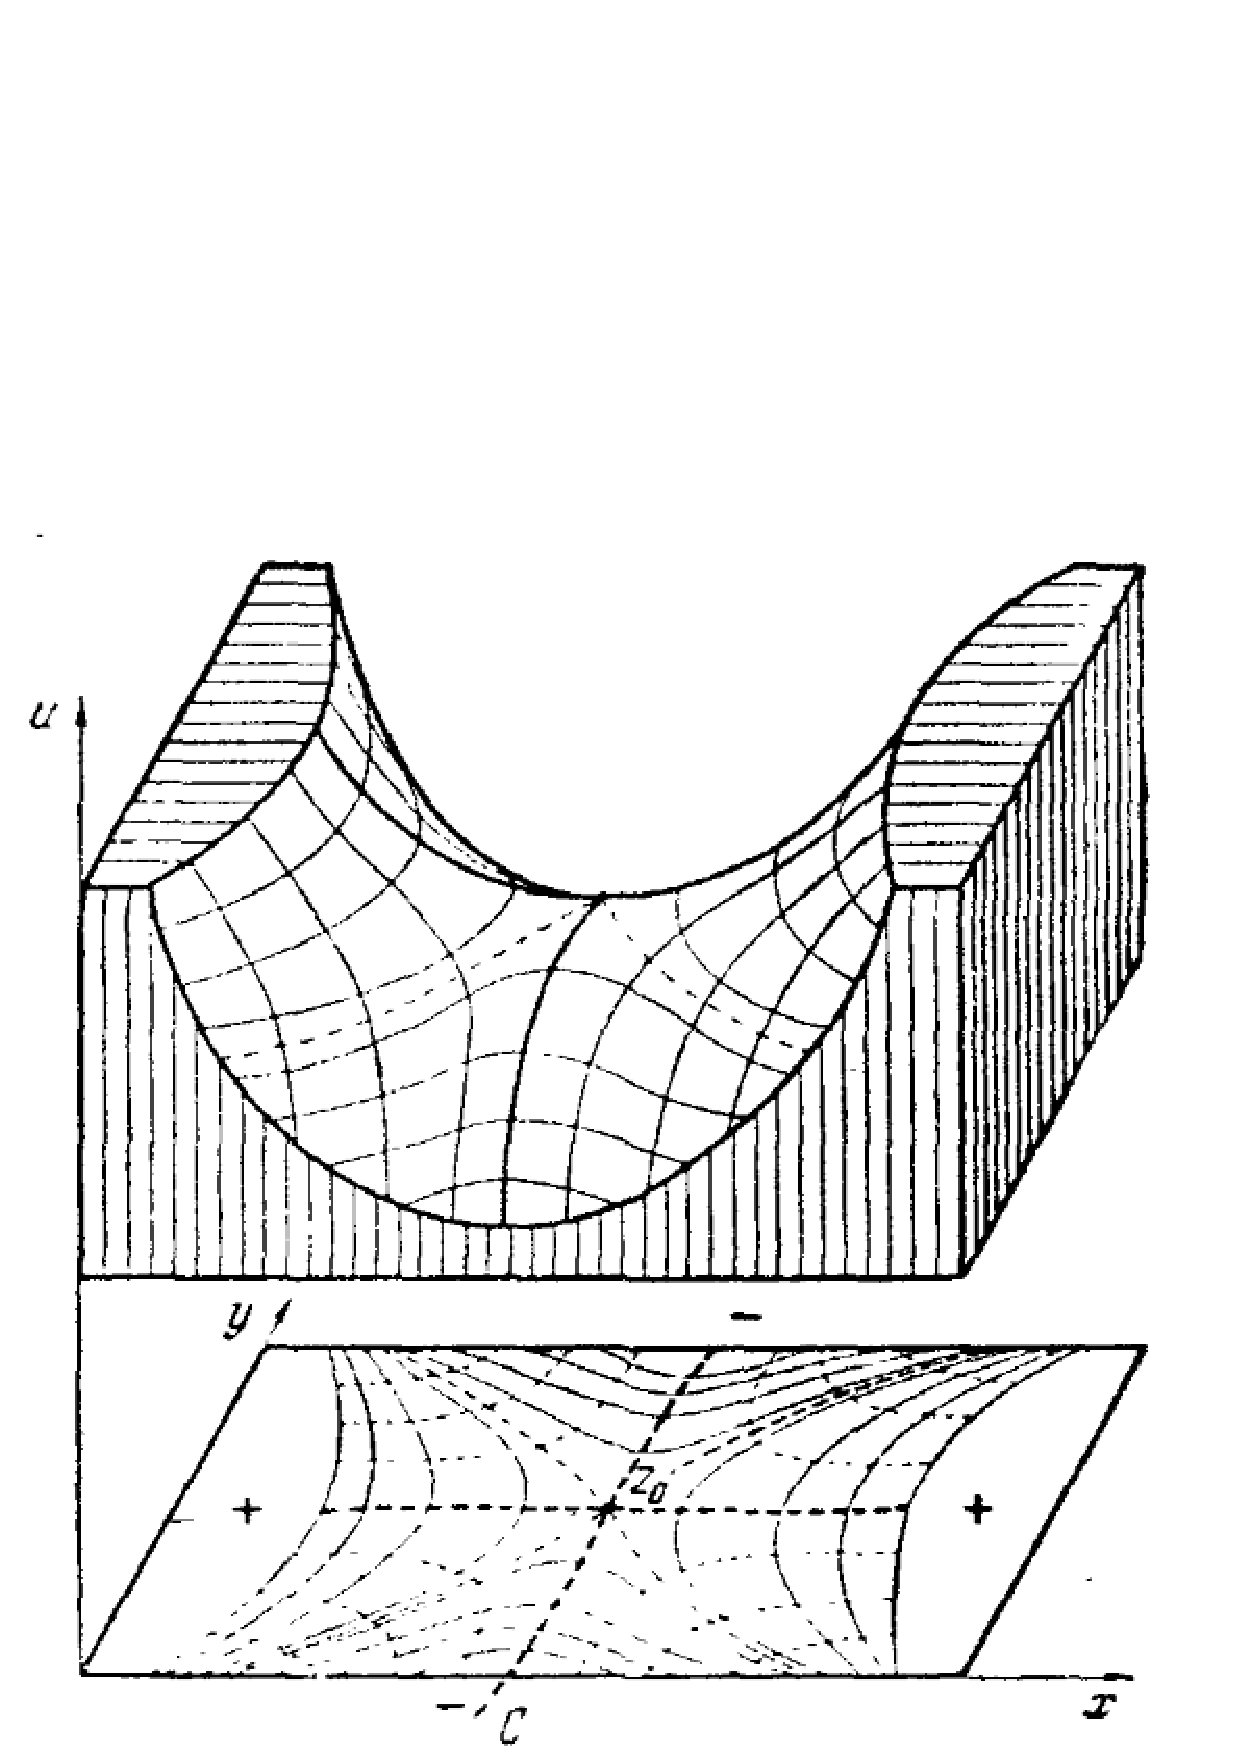
\includegraphics[width=0.3\linewidth]{pic2.png}}
	\caption{Седловые точки}
	\label{ris:image2}
\end{figure}

Наиболее удобный для оценки путь интегрирования $\widetilde{C}$, в каждой точке должен проходить в направлении наиболее быстрого изменения $\Re f(z)$, а так как функция f(z) аналитическая, то это направление должно совпадать с линией, на которой $\Im f(z) = \const$. 

Также, новый контур $\widetilde{C}$ должен содержать точку $z_0$, в которой $\Re f(z)$ достигает наибольшего значения на $\widetilde{C}$. Покажем для этого случая, что $f^\prime (z_0) = 0$, то есть точка линии $\Im f(z) = \const$, в которой $\Re f (z)$ достигает наибольшего значения, является точкой перевала.

Так и есть, ведь в точке $z_0$, которая является максимумом для $\Re f (z)$ производная $u=0$ вдоль линии $\widetilde{C}$ должна быть равна 0, т. е. $\frac{\partial}{\partial s}\Re f(z)=0$, а так как $\Im f(z) = \const$ на $\widetilde{C}$, то $\frac{\partial}{\partial s} \Im f(z) \equiv = 0$, а значит и 

$$
f^\prime(z_0) = \frac{\partial}{\partial s} \Re f(z) + i\frac{\partial}{\partial s} \Im f(z) = 0.
$$ 
  
\textit{Подведем итоги. Для метода перевала к интегралу (\ref{eq:eq6}) путь интегрирования $С$ следует деформировать в путь $\widetilde{C}$, проходящий через точку перевала $z_0$ и в окрестности этой точки идущий вдоль линии наибольшего ската $\Im f(z) = \const$ (рис. \ref{ris:image2}).}

Есть одно важное обстоятельство, обеспечивающее эффективность применения метода перевала: так как вдоль линии $\widetilde{C}$ имеем $\arg e^{f(z)} = \Im f(z) = \const$, то оценка интеграла (\ref{eq:eq6}) сводится к оценке интеграла от действительной функции, которая может быть проведена по методу Лапласа для интеграла вида (\ref{eq:eq7}).  

Именно это позволяет нам пользоваться полученными результатами теорем 1 и \ref{th:th2}. 

Рассмотрим  случай, когда путь интегрирования $С$ можно деформировать в путь $\widetilde{C}$, проходящий через точку перевала $z_0$, где $f^\prime(z_0) = 0$, $f^{\prime\prime}(z_0)\neq0$, и в окрестности $z_0$ совпадающий с линией наибольшего ската $\Im f(z) = \const$, причем на $\widetilde{C}$ вне этой окрестности $\Re f(z) < \Re f(z_0) - h \;(h> 0)$. Кроме того, предположим, что интеграл (\ref{eq:eq6}) абсолютно сходится для достаточно больших значений $\lambda$.
Тогда образом, оценку интеграла можно провести на основании теоремы 1. Пусть $z = z(t)$ будет уравнение контура $\widetilde{C}$; Тогда,

\begin{equation}\label{eq:eq11}
F(\lambda) = \int_{C}^{}\phi(z) e^{\lambda f(z)}dz=e^{\lambda i \Im f[z(t)]}\int_{a}^{b}\phi[z(t)]e^{\lambda \Re f[z(t)]}z^{\prime} dt
\end{equation}

задача сводится к оценки интеграла вида $\ref{eq:eq7}$ действительной области, разложение для которого уже было получено Лапласом, и имеет вид

$$
F(\lambda) = \int_{a}^{b}\phi(t)e^{\lambda f(t)}dt \sim \frac{e^{f(a)}}{\lambda}\sum_{n=0}^{\infty}\frac{n! c_n}{\lambda^n}
$$
  
Выпишем первый член этого разложения.\cite{Lavrentyev} Обозначим $\phi[z(t)]z^\prime = \widetilde{\phi}(t)$, $\Re f[z(t)] = \widetilde{f}(t)$ и тогда по формуле (\ref{eq:eq10}) получаем:

\begin{equation}\label{eq:eq12}
\int_{a}^{b} \widetilde{\phi}(t) e^{\lambda \widetilde{f}(t)}dt \sim e^{\lambda \widetilde{f}(t_0)} \sqrt{\frac{\pi}{\lambda}} \widetilde{c_0}
\end{equation}
где $\widetilde{c_0}$ - свободный член в разложении функции $\widetilde{\phi}[\widetilde{\psi}(\tau)]\widetilde{\psi^\prime}(\tau)$.

Имеем: $\widetilde{\phi}(t_0) = \phi(z_0) z^\prime (t_0)$, и исходя из того, что $f[z(t)] = \Re f[z(t)]+ i \Im f[z(t)] = \widetilde{f}(t)+\const$ вдоль $\widetilde{C}$, то

\begin{equation}\nonumber
\widetilde{f}^{\prime\prime} (t_0) = \frac{d^2}{d t^2} f[z(t)]\;|_{t=t_0} = f^{\prime\prime} (z_0) z^{\prime^2} (t_0).
\end{equation}
Причем $f^\prime[z(t)] z^{\prime \prime} (t) = 0$ при $t=t_0$. Так как эта величина отрицательна, то представив $z^\prime (t_0) = k e^{i \theta}$, можно записать ее в виде $\widetilde{f}^{\prime\prime}=-|f^{\prime\prime}(z_0)| k^2$. Получаем, что 

\begin{equation}\nonumber
\widetilde{c}_0=\widetilde{\phi}(t_0) \sqrt{-\frac{2}{\widetilde{f}^{\prime\prime}(z_0)}}= \phi (z_0) e^{i \theta} \sqrt{\frac{2}{|f^{\prime\prime}(z_0)|}}
\end{equation}
подставим найденное значение в (\ref{eq:eq12}), а затем в (\ref{eq:eq11}), получаем искомую формулу

\begin{equation}\label{eq:eq13}
F(\lambda) \sim e^{\lambda f (z_0)}\sqrt{\frac{2\pi}{|f^{\prime \prime} (z_0)|}} \phi(z_0) e^{i \theta} \frac{1}{\sqrt{\lambda}}
\end{equation}

Как уже много раз говорилось, точка $z_0$ - это точка, где $\Re f(z)$ достигает своего максимального значения. В то же время совершенно обычная ситуация - когда на искомом контуре $\widetilde{C}$ имеется несколько точек перевала, в которых значения $\Re f (z)$ находятся вблизи к наибольшему, то следует взять сумму выражений (\ref{eq:eq13}) по всем этим точками. 

Тот случай, когда контур интегрирования заканчивается в точке перевала $z_0$, аналогичным образом приводится к теореме \ref{th:th2}.

Итак, мы получили рабочую формулу, подставляя в которую составляющие наших искомых функций $\phi (z)$ и $f (z)$, мы должны получать приближенные значения интеграла, когда $\lambda \rightarrow \infty$ 

\section{Аппроксимация интеграла Бесселя}
\subsection{$\alpha<x$}
Попытаемся проверить полученную выше формулу. Возьмем интеграл Бесселя вида 

\begin{equation}\label{eq:eq14}
J_\alpha(x)=\frac{1}{2\pi}\int_{-\pi}^{\pi}e^{i(\alpha\tau-x\sin\tau)}d\tau
\end{equation} 
и найдем его разложение по формуле (\ref{eq:eq13})

Для начала нам необходимо найти точки перевала. Отметим тот факт, что у этого интеграла нет составляющей $\phi(t)$, то есть она равна 1, а функция $f(t)$ будет иметь вид 

\begin{equation}\nonumber
f(\tau) = \alpha \tau - x \sin \tau.
\end{equation} 

Найдем максимум этой функции $f(\tau)$

\begin{equation}\label{eq:eq15}
f^\prime(\tau) = \alpha - x \cos \tau = 0 \;\;\; \rightarrow \;\;\; \cos(\tau)=\frac{\alpha}{x}
\end{equation} 

Получаем, что $\tau = \pm \arccos\left(\frac{\alpha}{x} + 2\pi k \right), \;\;\; k \in \mathbb{N}$

Итак, получили много корей, но посмотрев на наш интервал $(0, 2\pi)$ замечаем, что на нем $\tau$ представлена двумя точками, но находить корни уравнения, когда они представлены в виде $\arccos\left(\frac{n}{x} + 2\pi k \right)$ неудобно. Поскольку функция четная, то мы можем перейти от решений уравнения $\alpha - x \cos \tau = 0$ на отрезке $(0, 2\pi)$ к решениям этого же уравнения на отрезке $(-\pi, \pi)$

Получили две перевальные точки

\begin{equation}\nonumber
\tau_{1,2} = \pm \arccos\left(\frac{\alpha}{x}\right)
\end{equation} 

Ранее было замечание о том, что если мы имеем несколько перевальных точек одного и того же уровня (находящихся достаточно близко), то для нахождения приближенного значения методом Лапласа нужно учитывать вклады всех этих точек, суммируя их.

Введем замену 
\begin{equation}\nonumber
\frac{\alpha}{x} = \vartheta
\end{equation}

Найдем необходимые элементы для подстановки в формулу (\ref{eq:eq13}). Для точки $\tau_1 = \arccos\vartheta$:

\begin{equation}\nonumber
f(\tau_1) = \alpha \arccos\vartheta - x \sin \arccos\vartheta = \alpha \arccos - x \sqrt{1-\vartheta^2}
\end{equation}

\begin{equation}\nonumber
\phi(z) \equiv 1
\end{equation}

\begin{equation}\nonumber
f^{\prime \prime} (\tau_1) = \sqrt{1-\vartheta^2}
\end{equation}

Аналогично находятся составляющие для точки $\tau_2 = -\arccos\vartheta$.

Получили формулу вида

\begin{eqnarray}\nonumber
J_\alpha(x) = \sqrt{\frac{1}{2 \pi x \sqrt{1-\vartheta^2}}} \left[ e^{i(\alpha \arccos 
	\vartheta - x \sqrt{1 - \vartheta^2} + \frac{\pi}{4})}  + e^{-i(\alpha \arccos 
	\vartheta - x \sqrt{1 - \vartheta^2} + \frac{\pi}{4})} \right]
\end{eqnarray}

Можем свернуть полученное выражение по формуле Эйлера:

\begin{eqnarray}\nonumber
J_\alpha(x) = \sqrt{\frac{2}{\pi x \sqrt{1-\vartheta^2}}} \cos \left[\alpha \arccos 
	\vartheta - x \sqrt{1 - \vartheta^2} + \frac{\pi}{4}\right]
\end{eqnarray}

Теперь сравним полученное приближение с известной функцией Бесселя. Для этого воспользуемся программным пакетом Maple:

Зафиксируем $\alpha=2$ и построим графики для $x$ на отрезке $(0, 30)$

\begin{figure}[h!]
	\center{\includegraphics[width=0.9\linewidth]{pic3.png}}
	\caption{Зависимость от $x$ ($\alpha=2$)}
	\label{ris:image3}
\end{figure}

Ранее говорилось, что этот метод применим для случая, когда значение параметров стремится к бесконечности, поэтому можно предположить, что этот пик в районе $x = 2$ связан с тем, что мы еще "недостаточно близки" к бесконечности. Однако, если мы зафиксируем $\alpha$ равным $15$, то полученный график  

\begin{figure}[h!]
	\center{\includegraphics[width=0.9\linewidth]{pic4.png}}
	\caption{Зависимость от $x$ ($\alpha=15$)}
	\label{ris:image4}
\end{figure}
дает нам понять, что дело не в этом. 

Вычтем графики, чтобы увидеть погрешность (рис. \ref{ris:image5}).

\begin{figure}[h!]
	\center{\includegraphics[width=0.9\linewidth]{pic8.png}}
	\caption{Погрешность при $\alpha=15$}
	\label{ris:image5}
\end{figure}

Можно заметить, что этот скачок наблюдается в том месте, где $\alpha \sim x$, а также то, что значения полученного приближения для случая, когда $\alpha > x$ совершенно не совпадают с искомой функцией. Но мы имеем очень хороший результат для случая $\alpha > x$, что тоже хорошо.

Аналогичную картину дает нам построение зависимостей от $\alpha$ при фиксированном $x$

Это отклонение от функции связано с выбором перевальных точек. Когда мы решали уравнение (\ref{eq:eq15}), то получили решение в виде арккосинуса для
$$
\cos(\tau)=\frac{\alpha}{x},
$$
но в случае если $\alpha>x$ мы получаем, что косинус больше единицы. Это возможно только в комплексной области, поэтому имеет смысл изменить решение этого уравнения.\cite{Wong}

\subsection{$\alpha>x$}

Посмотрим еще раз на уравнение (\ref{eq:eq13})
Ранее было сказано, что в наше случае порядок и аргумент болше 0, а значит, 
$$
\cos(\tau) \in (0;+\infty)
$$

Случай, когда косинус $\in (0; 1)$ был рассмотрен ранее, теперь посмотрим на остальной промежуток.
Косинус больше 1 только в том случае, если он имеет мнимую часть и не имеет действительную, исходя из этого можно сделать замену

$$
\tau = i t;
$$

Теперь уравнение принимает вид

$$
\cosh (\tau) = \frac{\alpha}{x}
$$

Выполняя обратную замену, получаем две точки 

$$
\tau_{\pm} = \pm i t_0
$$

где $t_0 = \arccosh \left(\frac{\alpha}{x}\right)$

Подставим полученные данные в $f(t)$

\begin{eqnarray}\nonumber 
f(\pm i t_0) = i (\alpha \tau - x \sin \tau) |_{\tau=\pm i t_0} = i (\alpha (\pm i t_0) - x \sin (\pm i t_0)) = \\
\nonumber= -(\pm \alpha t_0 \mp x \sinh(t_0)) = \mp(\alpha t_0 - x \sinh(t_0)) = \mp\alpha(t_0 - \tanh(t_0))
\end{eqnarray}

Найдем $f^{\prime \prime}(\pm i t{_0})$:

\begin{equation}\nonumber 
f^{\prime \prime}(\pm i t{_0}) = i x \sin (\pm i t_0) = \mp x \sinh (t{_0}) = \mp\alpha\tanh(t_0)
\end{equation}

Получили 2 перевальные точки. На оси $\tau$ функция 
$$
f(i t_0) = \mp \alpha (t_0 - \tanh(t_0))
$$
в этих точках функция достигает максимума в $\tau_0$ и минимума в $-\tau_0$. Легко видеть, что максимум на этом контуре интегрирования единственный (вытекает из рассмотрения производной). Исходя из полученных ранее замечаний следует, что основной вклад в значение функции несет перевальная точка, в которой $\Re f(t)$ максимальна, или близка к максимуму. Исходя из этих соображений, мы будем учитывать только точку $\tau_0$, пренебрегая вкладом $-\tau_0$.

Подставим полученные значения в (\ref{eq:eq13}).

\begin{equation}\label{eq:eq20}
J_\alpha(x) \sim \sqrt{\frac{1}{\alpha \tanh(t_0) 2 \pi}} e^{-\alpha(t_0 - \tanh(t_0))},
\end{equation}
где $t_0 = \arccosh(\frac{\alpha}{x})$

Нарисуем полученный график на рисунке (\ref{ris:image9})

\begin{figure}[h]
	\center{\includegraphics[width=0.5\linewidth]{pic9.png}}
	\caption{Приближение на $x \in (0; \alpha)$}
	\label{ris:image9}
\end{figure}



\subsection{Сливающиеся точки}
Итак, мы получили очень хорошее приближение для случаев $\alpha>x$, но остается неприятность в той самой точке $\alpha = x$. На самом деле эта ошибка связана с близостью перевальных точек.\cite{Fedoryuk} Для того же уравнения, в случае, если $\frac{\alpha}{x}$ близка к 1, получается функция, имеющая график вида(\ref{ris:image6})

\begin{figure}[h]
	\center{\includegraphics[width=0.5\linewidth]{pic5.png}}
	\caption{Перевальные точки (сливающиеся)}
	\label{ris:image6}
\end{figure}

В таком случае суммируя их вклады мы не получаем ничего хорошего, потому что вместо двух точек мы по факту получим одну. Однако в наших рассуждения было несколько важных допущений, как например то, что $f^{\prime} = 0$, в то время как в той точке между ними (в нуле) производная не равна нулю. Именно поэтому мы должны изменить наше приближение.

Разложим функцию $f(t)$ в ряд Тейлора в окрестности точки a. Можно заметить, что в нашем случае  $f^{\prime\prime}(t) = 0$

До этого мы использовали аналогичное разложение, но для хорошего порядка точности брали третье приближение (до второй производной), теперь , т.к. $f^{\prime\prime}(t) = 0$ мы столкнулись с тем, что нужно вернуть потерянную точность, поэтому будем использовать разложение вида:

\begin{equation}\label{eq:eq17}
f(t) \sim f(a) + \frac{f^{\prime}(a)}{1!}(t-a) + \frac{f^{\prime\prime\prime}(a)}{3!}(t-a)^3
\end{equation}

Заменим:

$$
a_1 = \frac{f^{\prime}(a)}{1!} \;\;\; a_3 = \frac{f^{\prime\prime\prime}(a)}{3!}
$$

Получаем:
  
\begin{equation}\label{eq:eq18}
f(t) \sim f(a) + a_1(t-a) + a_3(t-a)^3
\end{equation}
  
Теперь разложение интеграла (\ref{eq:eq14}) будет иметь вид

\begin{equation}\nonumber
J_\alpha(x) \sim \frac{1}{2\pi} e^{f(t_0)} \int_{-\pi}^{\pi}e^{a_1(t-t_0) + a_3(t-t_0)^3}dt
\end{equation}
где $t_0$ - середина между перевальными точками.

В нашем случае, $t_0=0$ (см. рис. \ref{ris:image5}), что заметно упрощает наш интеграл:

\begin{equation}\nonumber
J_\alpha(x) \sim \frac{1}{2\pi} f(t_0) \int_{-\pi}^{\pi}e^{a_1 t + a_3 t^3}dt
\end{equation}
  
Преобразуем его, заменив $a_3t^3 = \frac{t^3}{3} \rightarrow t = \left(\frac{1}{3a_3}\right)^{1/3}x$. Получаем:

\begin{equation}\nonumber
\int_{-\pi}^{\pi}e^{i\left(a_1 t + a_3 t^3\right)}dt = \int_{-\pi}^{\pi}e^{i\left(\frac{a_1}{(3a_3)^{1/3}}x + \frac{x^3}{3}\right)}dx 
\end{equation}

Заметим, что полученный интеграл почти полностью совпадает с функцией Эйри, имеющей вид:

\begin{equation}\nonumber
Ai(\alpha) = \frac{1}{2\pi}\int_{-\infty}^{\infty}e^{i\left(\alpha x + \frac{x^3}{3}\right)}dx 
\end{equation}

Но различаются пределы интегрирования. Как уже говорилось, при больших значениях $\lambda$ основной вклад в интеграл вносят перевальные точки, остальными же элементами можно пренебрегать. Поскольку наша точка находится в нуле, то пределы интегрирования могут быть растянуты от $(-\pi, \pi)$ до $(-\infty, \infty)$ без каких-либо последствий. Теперь можем заменить интеграл 
  
\begin{equation}\nonumber
	\int_{-\pi}^{\pi}e^{i\left(\frac{a_1}{(3a_3)^{1/3}}x + \frac{x^3}{3}\right)}dx = 2\pi Ai\left(\frac{a_1}{(3 a_3)^{1/3}}\right) \frac{1}{(3 a_3)^{1/3}}
\end{equation}

В итоге получаем готовое приближение интеграла Бесселя ($f(0)=0$)

\begin{equation}\label{eq:eq19}
J_\alpha(x) = Ai\left(\frac{(a_1)}{(3 a_3)^{1/3}}\right) \frac{1}{(3 a_3)^{1/3}},
\end{equation}
где $a_1=n-x\cos(0), \;\; a_2=\frac{x\cos(0)}{6}$

Сравним его с исходной функцией (рис \ref{ris:image7})

\begin{figure}[h!]
	\center{\includegraphics[width=0.5\linewidth]{pic6.png}}
	\caption{Приближение функцией Эйри, $\alpha=15$}
	\label{ris:image7}
\end{figure}

Итак, это приближение должно использоваться для случая, когда $\dfrac{\alpha}{x} \approx 1$. На графике видно, что при достаточных отклонения от точки $\dfrac{\alpha}{x} =1$ начинают появляться погрешности приближения. Построим график разности этих функций (рис. \ref{ris:image8})

\begin{figure}[h!]
	\center{\includegraphics[width=0.5\linewidth]{pic7.png}}
	\caption{Абсолютная погрешность}
	\label{ris:image8}
\end{figure}
  
На графике видно, что действительно, между перевальными точками ($x=15$) приближение полностью совпадает с искомой функцией. Чтобы избавиться от погрешностей около этой точки необходимо использовать полученные ранее формулы для случаев $\alpha>x$ и $\alpha<x$.  Но важно заметить, что нужно брать функцию для сливающихся точек в очень маленькой окрестности, то есть следить за точностью. Если возьмем ее на чуть большем интервале, то могут возникнуть серьезные отклонения.

Попробуем теперь объединить три полученных формулы приближения и сравнить их с функцией Бесселя (см. рис \ref{ris:image10}). 
  
\begin{figure}[h!]
	\center{\includegraphics[width=0.5\linewidth]{pic10.png}}
	\caption{Конечное приближение}
	\label{ris:image10}
\end{figure}

Для этого я построил 4 графика, 3 из которых - мои приближения на разных участках, выраженные кусочно-непрерывными функциями, а четвертый (синий) - есть функция Бесселя порядка 15. Заметим, что полученный график очень близок к искомой функции, и почти на всей оси достигается приемлемая точность, но на пике $x=17$ все равно осталась ощутимая погрешность, от которой в рамках перевальных оценок уйти нельзя.

\section{Заключение}
  
Нами была рассмотрена аппроксимация функций Бесселя методом перевала, сам метода перевала, а также границы его применимости. Полученные оценки оказались очень хорошими. 

Аналогичными способами можно приближать большое количество интегралов вида \ref{eq:eq6}, которые, как уже говорилось ранее, могут появиться при описании (исследовании) разнообразных явлений природы. Но, как ранее было замечено, нужно аккуратно оценивать функции на возникновение аномалий в точках перехода. Очень важным является выбор интервалов для использования различных приближений, поэтому обязательно строить графики для оценки погрешностей и подбирать границы этих интервалов. 

Да, метод Лапласа, который используется для этих оценок оставляет небольшие погрешности. Это не очень плохо, ведь чаще всего этот метод  дает оценку, точнее которой в разумное время получить невозможно. Но он дает нам готовую формулу для вычисления такого сложного для вычисления интеграла. Готовая формула дает нам легко оценивать зависимость системы от различных параметров, что очень удобно. 

Тот огромный прирост к скорости, который дает нам эти оценки иногда могут играть очень важную роль при различного вида исследования. Но нужно понимать, что эти, казалось бы малые погрешности, могут для ряда задач оказаться чрезвычайно негативным фактором, и придется от них отказаться.
 
\newpage
\bibliographystyle{utf8gost705u}  %% стилевой файл для оформления по ГОСТу
\bibliography{biblio}     %% имя библиографической базы (bib-файла) 
\end{document} 